\cleardoublepage \phantomsection
\addcontentsline{toc}{chapter}{Introduction}
\chapter*{Introduction}

This document describes the process of understanding and designing a computational tool for the simulation of electromagnetic waves in periodic crystals. It gives account of the  theory and concepts that are necessary for modeling electromagnetic fields using the Finite Element Method (FEM), and goes further by presenting the approach we used to implement it in the form of a software platform based in the Object Oriented Programming Paradigm. The document concludes by showing a set of results from simulations obtained by using the program, and compares these to analytic solutions and also to Photonic Crystal simulations taken from the literature. Good agreement with the references is found, and the software platform proved to be a promising tool for the modeling of photonic crystal devices.

The project is thus, framed in the context of a field known as computational electromagnetism, which can bee seen as an intersection between the theory of Electromagnetic Physics, the mathematics of numerical methods and application of techniques and devices product of computer science. All of this together, gives rise to the computational platforms that enable engineers to model, design, and test novel electromagnetic components before actually making them. Saving thus, production costs and optimizing functionality.  
\begin{figure}
\centering
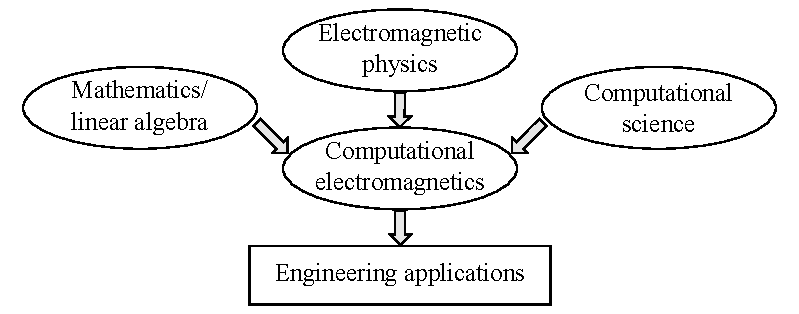
\includegraphics[scale=1]{./img/interdisciplinary.pdf}
\caption{Computational electromagnetism is a highly interdisciplinary field. Taken from \cite{Jin2010}}
\label{fig:computational}
\end{figure}
In our case, the novel technology that the tool we design is allowing to test is that of \textbf{Photonic Crystals}. Photonic Crystals are materials designed to have light manipulation properties capable of revolutionizing the field of telecommunications and signal processing. With them, we can design devices that are able to confine, and mold light (like in figure \ref{fig:guide_point}) in ways that are similar to how electronic circuits manipulate charges and currents.  Opening the doors to realizable photonic circuits and new technologies.

\begin{figure}
\centering
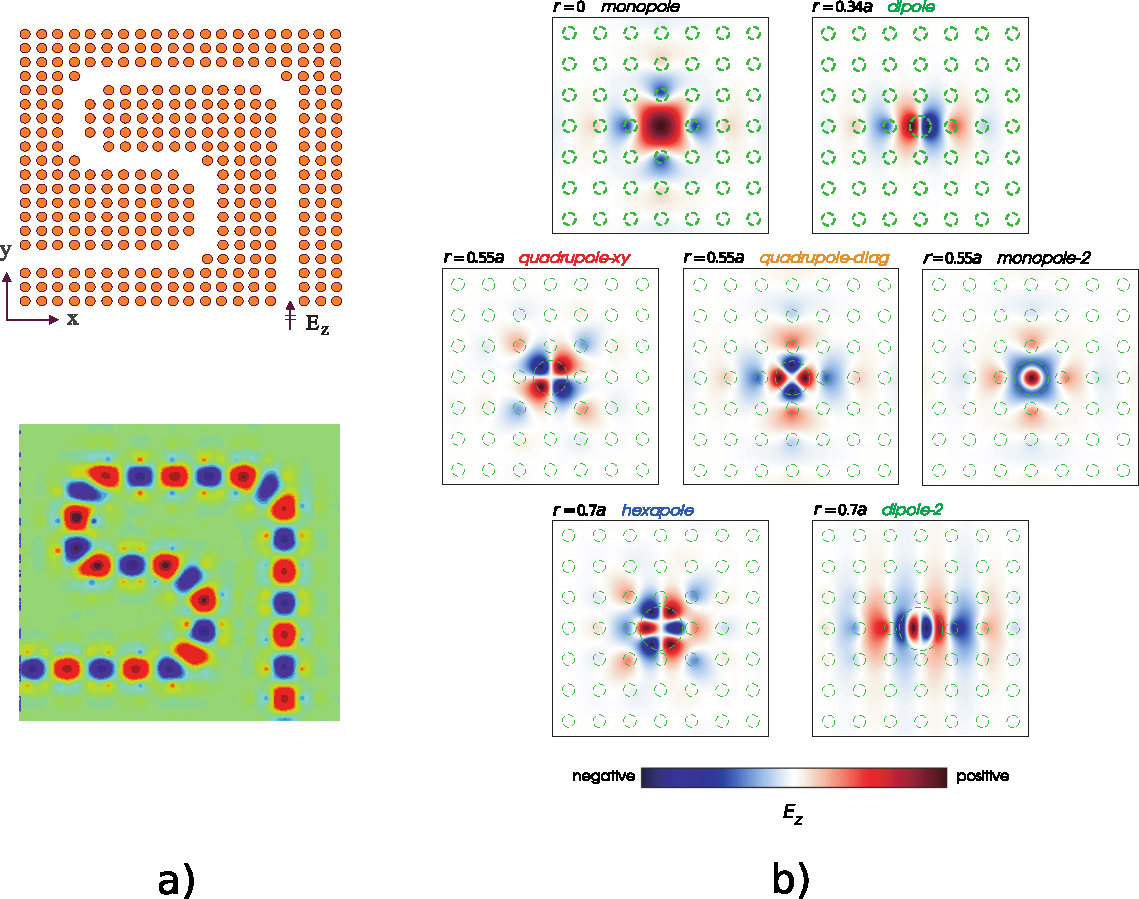
\includegraphics[scale=0.7]{./img/pcs.pdf}
\caption{a) Line defects acting as a wavegide \cite{Jin2010}. b) Point defects where resonant modes are confined \cite{Joannopoulos2008}.}
\label{fig:guide_point}
\end{figure}
